\documentclass[tikz,border=6pt]{standalone}
\usepackage{amsmath,amssymb}
\begin{document}
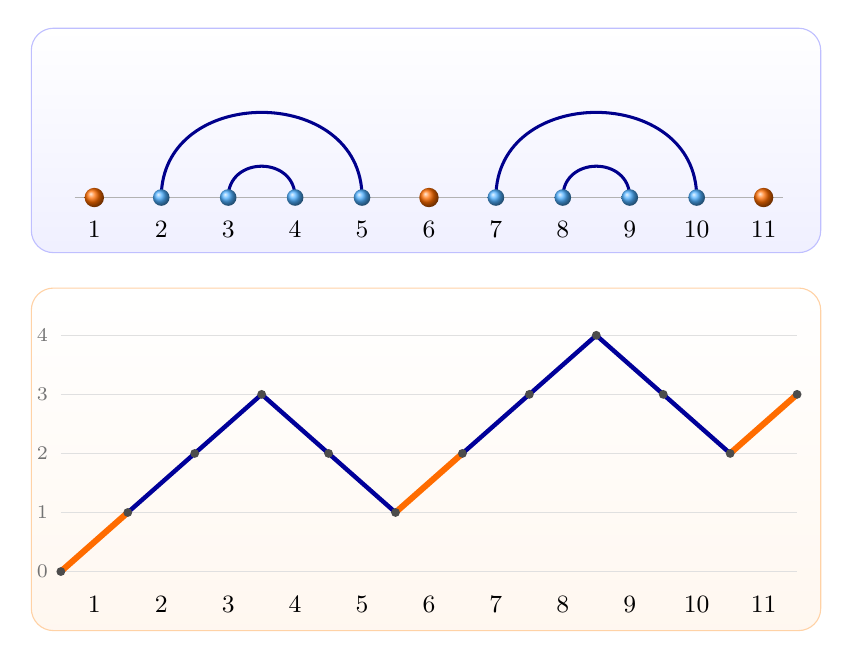
\begin{tikzpicture}[
  arcpt/.style={circle,shading=ball,ball color=blue!45!cyan!70,inner sep=0pt,minimum size=6pt},
  freept/.style={circle,shading=ball,ball color=orange!85!red,inner sep=0pt,minimum size=7pt},
  arcl/.style={draw=blue!55!black,line width=1.1pt},
  up/.style={draw=blue!60!black,line width=1.6pt,line cap=round},
  upfree/.style={draw=orange!85!red,line width=2.2pt,line cap=round},
  down/.style={draw=blue!60!black,line width=1.6pt,line cap=round},
  lbl/.style={font=\small}]
\def\dx{0.85}
% top: points and arcs
\shade[rounded corners=8pt,top color=white,bottom color=blue!6,draw=blue!25] (0.05,-0.7) rectangle (11.5*\dx+0.3,2.15);
\draw[black!30,line width=0.5pt] (\dx-0.25,0) -- (11*\dx+0.25,0);
\draw[arcl] (2*\dx,0) to[out=90,in=90,looseness=1.45] (5*\dx,0);
\draw[arcl] (3*\dx,0) to[out=90,in=90,looseness=1.6] (4*\dx,0);
\draw[arcl] (7*\dx,0) to[out=90,in=90,looseness=1.45] (10*\dx,0);
\draw[arcl] (8*\dx,0) to[out=90,in=90,looseness=1.6] (9*\dx,0);
\foreach \i in {2,3,4,5,7,8,9,10} \node[arcpt] at (\i*\dx,0) {};
\foreach \i in {1,6,11} \node[freept] at (\i*\dx,0) {};
\foreach \i in {1,...,11} \node[lbl,below=5pt] at (\i*\dx,0) {$\i$};
% bottom: the nonnegative sequence
\begin{scope}[yshift=-4.75cm]
  \shade[rounded corners=8pt,top color=white,bottom color=orange!6,draw=orange!35] (0.05,-0.75) rectangle (11.5*\dx+0.3,3.6);
  \foreach \h in {0,...,4} {
    \draw[black!12,line width=0.4pt] (0.5*\dx,\h*0.75) -- (11.5*\dx,\h*0.75);
    \node[font=\scriptsize,black!55,anchor=east] at (0.5*\dx-0.04,\h*0.75) {$\h$};
  }
  \foreach \i/\a/\b in {1/0/1,2/1/2,3/2/3,4/3/2,5/2/1,6/1/2,7/2/3,8/3/4,9/4/3,10/3/2,11/2/3} {
    \pgfmathsetmacro{\xa}{(\i-0.5)*\dx}\pgfmathsetmacro{\xb}{(\i+0.5)*\dx}
    \ifnum\i=1 \draw[upfree] (\xa,\a*0.75) -- (\xb,\b*0.75);
    \else\ifnum\i=6 \draw[upfree] (\xa,\a*0.75) -- (\xb,\b*0.75);
    \else\ifnum\i=11 \draw[upfree] (\xa,\a*0.75) -- (\xb,\b*0.75);
    \else \draw[up] (\xa,\a*0.75) -- (\xb,\b*0.75);
    \fi\fi\fi
  }
  \foreach \i/\b in {0/0,1/1,2/2,3/3,4/2,5/1,6/2,7/3,8/4,9/3,10/2,11/3}
    \fill[black!70] (\i*\dx+0.5*\dx,\b*0.75) circle (1.6pt);
  \foreach \i in {1,...,11} \node[lbl] at (\i*\dx,-0.42) {$\i$};
\end{scope}
\end{tikzpicture}
\end{document}
